% !TEX program = pdflatex
\usepackage{amstext}
\usepackage{amsmath}
\usepackage{graphicx}
\usepackage{float}
\usepackage{varioref}
\usepackage[final]{pdfpages}
\usepackage{fancyref}
\usepackage[section]{placeins}
\usepackage{perpage}
\usepackage{caption}
\usepackage{comment}
\usepackage{appendix}
\usepackage{verbatim}
\usepackage{epstopdf}
\usepackage[english]{babel}
\usepackage{hyperref}
\usepackage{dsfont}
\usepackage{booktabs}
\usepackage{minted}
\usepackage{subcaption}
%\usepackage{fixltx2e}
\usepackage{ulem}
\usepackage[margin=1in, paperwidth=8.5in, paperheight=11in]{geometry}
\usepackage[section]{placeins} %makes your figures not float past section barriers
\usepackage{perpage} %restarts footnote numbering by page
\MakeSorted{figure} %deals with figures using both [!ht] and [!ht]
\vrefwarning % Makes sure your document compiles when you screw up the references
\hypersetup{
    colorlinks=true,
    linkcolor=blue,
    filecolor=magenta,      
    urlcolor=cyan,
}


\title{Wireless Comms Lab 1}
\author{
        Evan Dorsky \\
        Forrest Bourke
}
\date{\today}

\documentclass[12pt]{article}

\begin{document}
\maketitle

\begin{abstract}
This report contains a block diagram of our system, plots of transmitted and received signals (before and after timing synchronization), a complete description of the timing synchronization algorithm we used and our achieved data rate.
\end{abstract}

\section{Block Diagram}
This is time for all good men to come to the aid of their party!

\section{Signals}
\subsection{Transmitted}
\begin{figure}[!ht]
\centering
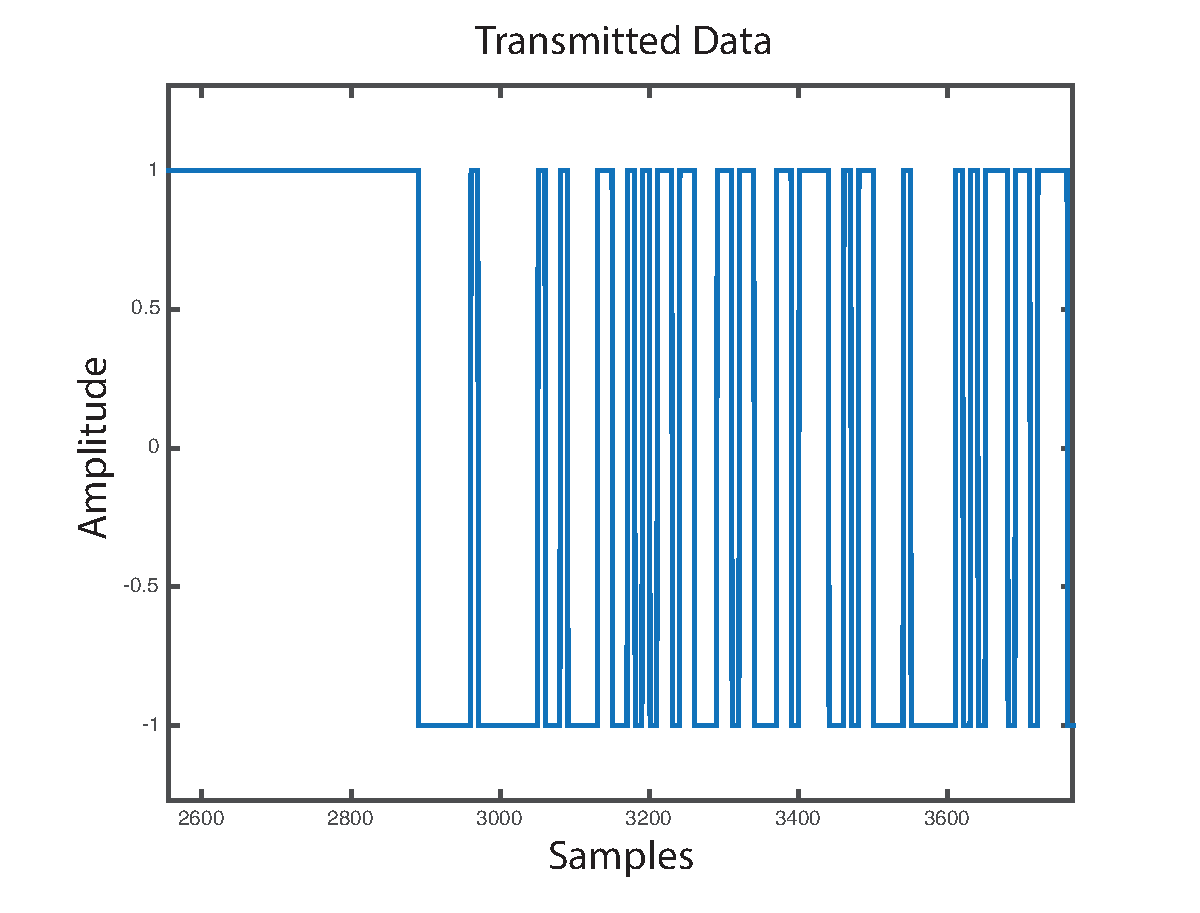
\includegraphics[width=.8\textwidth]{tx.eps}
\caption{Transmitted Data}
\label{fig:tx}
\end{figure}
    
\subsection{Received}

\section{Timing Synchronization}



\end{document}
This is never printed
